\documentclass[tikz,border=12pt]{standalone}
\usepackage{amsmath,amssymb}
\usepackage{tikz}
\usetikzlibrary{arrows.meta,positioning,fit,calc,shapes.geometric}

\definecolor{driftC}{HTML}{1F4E79}
\definecolor{coupC}{HTML}{0B6E4F}
\definecolor{driveC}{HTML}{8B3A3A}
\definecolor{bgSoft}{HTML}{F7F5F1}
\definecolor{ink}{HTML}{1A1A1A}

\begin{document}
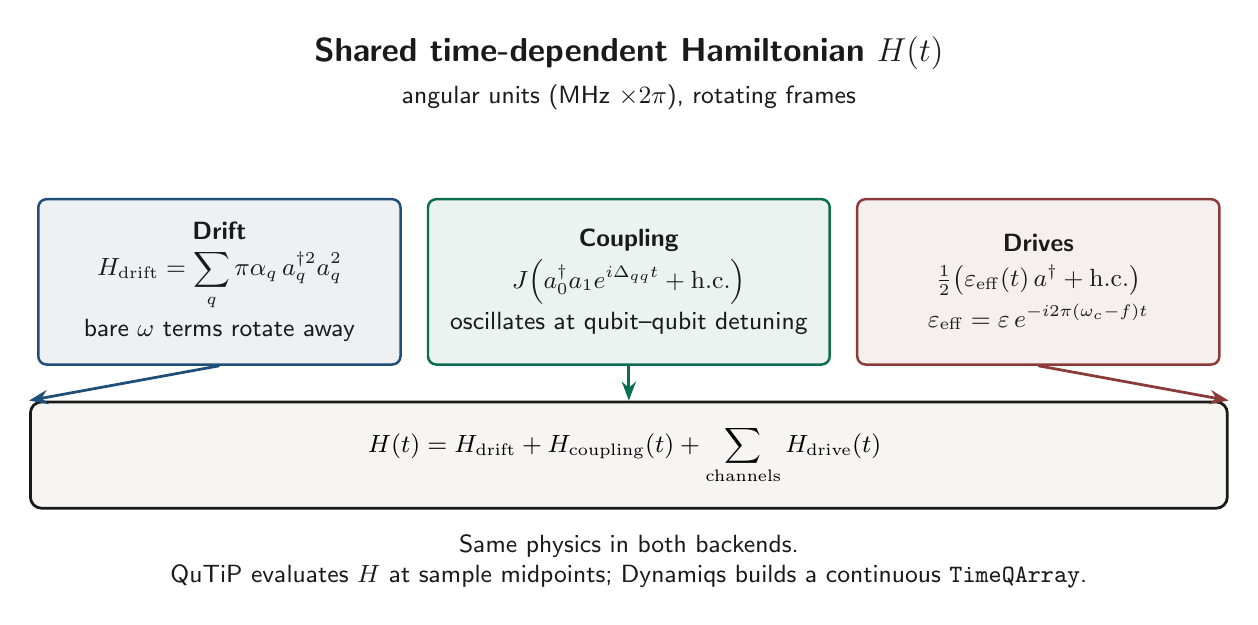
\begin{tikzpicture}[
  font=\sffamily\small,
  box/.style={
    draw=#1, line width=0.9pt, rounded corners=3pt,
    fill=#1!8, align=center, inner sep=8pt, text=ink,
    minimum width=4.6cm, minimum height=2.1cm
  },
  title/.style={font=\sffamily\bfseries\large, text=ink},
  eq/.style={font=\sffamily\small, text=ink},
  >={Stealth[length=2.4mm]}
]

\node[title] (T) at (0,4.1) {Shared time-dependent Hamiltonian $H(t)$};
\node[eq] (sub) at (0,3.55) {angular units (MHz $\times 2\pi$), rotating frames};

\node[box=driftC] (D) at (-5.2,1.2) {%
  \textbf{Drift}\\[2pt]
  $H_{\mathrm{drift}}=\displaystyle\sum_q \pi\alpha_q\,a_q^{\dagger 2}a_q^{2}$\\[2pt]
  bare $\omega$ terms rotate away
};

\node[box=coupC] (C) at (0,1.2) {%
  \textbf{Coupling}\\[2pt]
  $J\!\left(a_0^{\dagger}a_1 e^{i\Delta_{qq}t}+\mathrm{h.c.}\right)$\\[2pt]
  oscillates at qubit--qubit detuning
};

\node[box=driveC] (R) at (5.2,1.2) {%
  \textbf{Drives}\\[2pt]
  $\tfrac12\!\left(\varepsilon_{\mathrm{eff}}(t)\,a^{\dagger}+\mathrm{h.c.}\right)$\\[2pt]
  $\varepsilon_{\mathrm{eff}}=\varepsilon\,e^{-i2\pi(\omega_c-f)t}$
};

\node[draw=ink, line width=1pt, rounded corners=4pt, fill=bgSoft,
      minimum width=15.2cm, minimum height=1.35cm, align=center]
  (H) at (0,-1.0) {%
  $H(t)=H_{\mathrm{drift}}+H_{\mathrm{coupling}}(t)+\displaystyle\sum_{\mathrm{channels}}H_{\mathrm{drive}}(t)$
};

\draw[->, line width=1pt, driftC] (D.south) -- (H.north west);
\draw[->, line width=1pt, coupC] (C.south) -- (H.north);
\draw[->, line width=1pt, driveC] (R.south) -- (H.north east);

\node[eq, align=center] at (0,-2.35) {%
  Same physics in both backends.\\
  QuTiP evaluates $H$ at sample midpoints; Dynamiqs builds a continuous \texttt{TimeQArray}.
};

\end{tikzpicture}
\end{document}
